% Write the full path to the location of the graphics relative to book.tex
\graphicspath{{chapters/parsons/graphics/}}

\title{Function Scaling and Adaptive Boundary Condition Throttling for
  Convergence Control in Highly Nonlinear Poisson--Boltzmann
  Electrolyte Models.}
\titlerunning{Function Scaling and Adaptive Convergence Throttling}

\author{Drew~F.~Parsons, Matteo~Farci,  Alin~Grigoras, and Dagmawi Tadesse}
\authorrunning{Parsons et al.}

\institute{D.~F.~Parsons \email{drew.parsons@unica.it}
  \and M.~Farci \and A.~Grigoras
  \at 
Department of Chemical and Geological Sciences, University of Cagliari, Cagliari, Italy,
\and Dagmawi Tadesse
\at School of Mathematics, Statistics, Chemistry and Physics, Murdoch University, Murdoch, WA, Australia
}

\maketitle

\abstract{The Poisson--Boltzmann (PB) model of electrolyte solutions
combines the Poisson equation for electrostatic potentials with a
Boltzmann equation $c = c_0 \exp[-e\psi/kT]$ for mobile ion
concentrations that is highly nonlinear once the electrostatic
potential exceeds 0.1 V. This introduces numerical
challenges: first, suitable convergence conditions for the
concentration functions become sensitive to the boundary
potential. Second, a controlled initial guess must be provided to
avoid the finite element method calculation diverging to NaN. We
resolve the first challenge by logarithmically scaling the
concentration function.  A nontrivial log-zero scaling function can handle
the near-zero concentrations of coions in a classical point charge
model, though is redundant in an advanced model that includes steric
forces due to finite ion sizes.  The second challenge is resolved with
an adaptive throttling algorithm that throttles large values of
boundary conditions down to the level of the linear regime and then
iteratively raises the throttle until the final nonlinear solution is
obtained.
The combination of a steric model and throttling enables computation of
concentrated electrolytes with electrode potentials as high as 2,000
V. We provide a general derivation of the weak and strong forms of the
 PB system from the underlying thermodynamic energy functional. } 

\section*{Introduction}

Continuum theory (mean field theory) has been an effective tool for
studying the behaviour of systems in electrolyte solutions. The
Poisson--Boltzmann (PB) model \citep{Wu2022} enables evaluation of ion
adsorption layers at surfaces together with the electric field generated by surface charge and adsorbed ions. The PB model underpins
the theory of stability of microparticle suspensions in aqueous media,
enabling the modelling of particle aggregation and surface forces. The
same theory can also be applied to model electrochemical
systems, including energy storage devices, batteries, or
supercapacitors. However, there is a crucial difference in the two classes
of applications that has a significant impact on the numerical
stability of the model.  The surface potentials
of typical microparticles, such as protein molecules or metal oxide
particles, tend to lie in the range 5--50 mV, which is 0.2--2
$kT$ in thermal energy units (based on a thermal potential at $T=298$
K defined by $e\psi_{T} = kT$, where $e$ is the elementary charge, $k$
is Boltzmann's constant, and $T$ is temperature). Electrolytic energy
storage systems, by contrast, typically operate with electrode
potentials on the order of 1--5 V, that is, 1,000--5,000 mV, or 40--200
$kT$.  The nonlinearity of the PB model is highly
sensitive to energies exceeding one $kT$ unit, requiring particular
algorithms to enable numerical nonlinear convergence.  Our goal is to
set up the calculation to solve successfully over a broad range of
electrode potentials without requiring the manual readjustment of
convergence parameters.  We identify two main steps, implemented via
finite element methods using FEniCSx \citep{baratta2023dolfinx}: the log scaling of
ion concentration functions and the adaptive throttling of boundary
conditions.

For context, we first present a summary of the physics and
derive the
weak and strong formulations defining the PB model from
the underlying thermodynamic energy functional. The derivation
is general, allowing for spatially varying permittivity, although we
employ a dielectric constant in the calculations here. The derivation
allows for non-electrostatic interactions of the electrolyte, 
particularly steric forces due to finite ion size effects.  
To focus on the numerical algorithms, we omit redox
phenomena (including the electrolysis of water) that would occur in real
systems at high electrode potentials.

\section{Weak Formulation of the PB Model}

The energy functional for an electrolyte solution determined by
electrostatic potential $\psi(x)$ and ion concentration profiles
$c_i(x)$ can be composed from various fundamental energy
contributions, as follows:
\begin{equation}
    \Omega[\psi, c_i] = \Omega_{el} + \Omega_{en} +  \Omega_{ex},
\end{equation}
where $\Omega_{el}$ describes the direct energy of the electrostatic field generated by the electric charge of ions and surfaces \citep{Jackson_Classical_Electrodynamics}:
\begin{equation}
  \Omega_{el}  =\frac{1}{2} \int_{V}D \cdot E dx
  = -\frac{1}{2} \int_{V}D \cdot E dx + \sum_i \int_V z_i e c_i(x) \psi(x) dx
  + \int_{S} \sigma(s) \psi(s) ds,
\end{equation}
with $E$ denoting the electric field, $E=-\nabla\psi$; $D$ the
electric displacement, $D=\varepsilon_0
\varepsilon(x)E$; $\varepsilon_0$ the permittivity of the vacuum;
 $\varepsilon(x)$ the (spatially varying) relative
permittivity; $z_i$ the valency of ion $i$; and $\sigma(s)$ the
surface charge density on boundary $S$. Here, $V$ refers to the domain
(volume) of the system in space.

The term $\Omega_{en}$ describes the ideal entropic energy of ions, treated as ideal (non-interacting) particles \citep{GrayStiles2018,DagmawiParsons2024}:
\begin{equation}
    \Omega_{en} = kT \sum_{i} \int_{V} \left[ c_i(x) \ln \left(\frac{c_i(x)}{c_{i\infty}} \right) - c_{i}(x) + c_{i\infty} \right] dx,
\end{equation}
where $c_{i\infty}$ is the bulk concentration of ions. As a point of
physics, it is important to note that the use of a fixed bulk
concentration means the system is controlled by the chemical potential
of ions, with a variable number of ions in the domain $V$ of interest.
In other words, the thermodynamic potential is a grand potential, not 
(Helmholtz) free energy, and for that reason we write the energy as $\Omega$ rather
than $F$. A free energy formulation (with a fixed number of ions) would
require the use of a thermal de Broglie wavelength instead of
$c_{i\infty}$ \citep{GrayStiles2018}.


The grand potential term $\Omega_{el} + \Omega_{en}$ defines the conventional
PB model. The term $\Omega_{ex}$ represents extra
contributions to the total energy functional that describe other
relevant physics, such as pH-dependent charge regulation
\citep{ParsonsSalis2019}, specific ion interactions
\citep{ParsonsCarucciSalis2022}, or steric forces due to finite ion
size \citep{LopezGarciaHornoGrosse2018}. We consider the latter in this
work.

The PB model describes the system in equilibrium,
obtained by minimizing the total grand potential with variation
$\delta\Omega=0$ with respect to $\psi$ and $c_i$. Variation with
respect to $\psi$ (with a test function $p \equiv \delta \psi$) leads to a weak formulation
for the Poisson equation
\begin{equation}
    0 = -\int_{V} \varepsilon_{0}\varepsilon(x) (\nabla\psi,\nabla p) dx + \sum_{i}z_i e \int_{V} c_{i}(x) p dx + \int_{S_{N}} \sigma(s) p ds
    \label{weak_Poisson}
\end{equation}
for all test functions $p$ in the relevant function space (vanishing
on the Dirichlet boundary subdomain $S_{D} \subset S$).  A Dirichlet boundary
condition $\psi(x)=\psi_{0}$ for $x \in S_{D}$ can be applied to set a defined potential,
for instance, the potential of an electrode controlled by a
potentiostat. For other boundary subdomains $S_{N} = S \setminus
S_{D}$, a Neumann boundary condition can be set via the surface
charge density $\sigma$ in the surface term, applying Gauss' law at
the external boundary,\footnote{At an internal boundary, $\sigma=D^{\text{out}}_{\perp}-D^{\text{in}}_{\perp}$.}
\begin{equation}
  \sigma = -D_{\perp} = (n, \varepsilon_{0}\varepsilon\nabla \psi),
  \label{surface_charge_gauss}
\end{equation}
where $D_{\perp}$ is the transverse component of the electric
displacement vector $D$ at the boundary, or, equivalently, $n$ is the
outward normal vector at the boundary. Here, \eqref{surface_charge_gauss}
is valid across the entire  external surface $S$ but sets a Neumann
boundary condition when applied to the surface subdomain
$S_{N}$ in \eqref{weak_Poisson}. Applied at $S_{D}$, \eqref{surface_charge_gauss} evaluates the surface charge density generated at Dirichlet surfaces.
After additional
integration by parts, the weak formulation \eqref{weak_Poisson} leads to the strong
formulation of the electrostatic Poisson equation,
$\nabla\cdot D = \sum_i z_i e c_{i}(x)$.

The variation of $\Omega$ with
respect to each ion concentration profile $c_i$ (in turn, with test
functions $b_i\equiv \delta c_i$), assuming linear variations such that
$\ln(1+b_i/c_i)\approx b_i/c_i$, leads to the weak formulation of Boltzmann's
equation,
\begin{equation}
    0 = \int_{V} \left[ e z_i \psi(x)
    + kT \ln\left(\frac{c_i(x)}{c_{i\infty}}\right)
  \right] b_i dx,
    \label{weak_Boltzmann}
\end{equation}
for all test functions $b_i$. The strong form of the classical
Boltzmann equation, $c_i(x)=c_{i\infty}\exp(-z_i
e \psi(x)/kT)$, can then be obtained.  The Boltzmann equation is implicitly controlled by
the bulk concentrations $c_{i\infty}$, and an explicit boundary condition
for the concentration functions is not needed.

\subsection{Non-electrostatic Interactions: A Steric Model with  Finite Ion Size}

In the classical point charge PB model, the
ion concentrations $c_i$ are determined completely by the
electrostatic potential with the Boltzmann equation in closed form,
such that
only the Poisson equation would need to be solved directly. However, the
physical problem with the classical model is evident in electrochemical
systems with an electrode potential of 1 V. A 1 V potential is
equivalent to a thermal energy of $40 kT$ (at room temperature), for which the conventional
Boltzmann factor for a counterion is
$\exp(40)\approx 2.3 \times 10^{17}$.  That is, the surface counterion
concentration of a 1M electrolyte would exceed $10^{17}$ mol/L, which
is clearly unphysical.  We return the model to physical
relevance by adding an extra steric energy term $\Omega_{ex}$ with
corresponding excess chemical potential per ion $\mu_{i}^{ex}$, for
which the modified Boltzmann equation is
\begin{equation}
    c_i(x)=c_{i\infty}\exp\left[(-(z_i e \psi(x) + \mu_i^{ex}(x)-\mu_{i\infty}^{ex})/kT\right].
    \label{general_Boltzmann}
\end{equation}
This corresponds to a total chemical potential $\mu_i(x)$ for each ion,
defined by
\begin{eqnarray}
  \mu_i(x) &=& \mu_{i}^{\textrm{entropic}} +  \mu_{i}^{\textrm{electrostatic}} +
               \mu_{i}^{ex} \\
{} &  =&\mu_{i\infty} + kT \ln(c_i(x)/c_{i\infty})
         + ez_i \psi(x) + \mu_i^{ex}(x)-\mu_{i\infty}^{ex},
         \label{chem_pot}
\end{eqnarray}
where $\mu_{i\infty}$ refers to the (fixed) excess chemical potential of the
ion in bulk solution, defined relative to an ideal unit
reference solution by $\mu_{i\infty} = kT\ln c_{i\infty} + \mu_{i\infty}^{ex}$.
The steric model we employ is the Carnahan--Starling \citetext{CS, \citeyear{CarnahanStarling1969}} model,
 with a contribution to the grand potential
% for future reference, the CS model (both energy and chemical
% potential)  can be considered as Padé approximations
% i.e. rational  polynomials functions
% which give good convergence when used in the Homotopy Series Method
% thus tells us Liao
\begin{equation}
    \Omega_{ex} = \sum_{i} \int_{V} c_{i}(x) \left[ kT
    \frac{4\phi - 3\phi^2}{(1-\phi)^2}
    -  \mu_{i\infty}^{ex}
  \right]dx
  \label{CS_energy_functional}
\end{equation}
and the weak formulation
\begin{equation}
    0 = \int_{V} (\mu_i^{ex}-\mu_{i\infty}^{ex}) b_i \, dx
    \label{weak_CS}
\end{equation}
for all $b_i$, which is added to \eqref{weak_Boltzmann}, the weak
formulation for the Boltzmann equation, together generating the strong
formulation of the modified Boltzmann
equation, \eqref{general_Boltzmann}.  Here the excess chemical potential
per ion for the CS model, corresponding to the energy
functional \eqref{CS_energy_functional}, is
\begin{equation}
    \mu_{i}^{ex} = kT \frac{\phi(8-9\phi+3\phi^2)}{(1-\phi)^3},
    \label{chem_pot_CS}
\end{equation}
where $\phi$ is the \emph{total} ion volume fraction defined by
$\phi=\sum_i c_i v_i$, with $v_i$ the intrinsic molar volume per
ion $i$. Hence the CS excess chemical potential is defined identically
for all ions. 

To derive the weak formulation in \eqref{weak_CS}, we
applied a homogenized component approximation that assigns common
volumes at the point of introducing the variation  $\delta c_i$ (i.e.\
the test function $b_i$), such that $\delta\phi=v_j \delta c_i$ rather 
than $v_i \delta c_i$. This approximation is required since the CS
model was formulated for single-component systems. The more complex
multicomponent Boublík--Mansoori--Carnahan--Starling--Leland model would enable ion-specific chemical
potentials \citep{MansooriCarnahanStarlingLeland1971}, removing the
need for this approximation. The terms $\phi_{\infty}$, $\mu_{i\infty}^{ex}$
are the bulk total volume fraction and excess chemical potential
defined by bulk concentrations $c_{i\infty}$. With this term, the
Boltzmann equation \eqref{general_Boltzmann} becomes transcendental in $c_i$, precluding a closed
expression that would determine ion concentrations. Concentration functions must therefore be
explicitly solved  numerically alongside the potential $\psi$. In this
paper, we address strategies for managing the strong nonlinearity in
the system introduced by this term in the presence of large values of the
potential. Note that $c_i$ must also be solved explicitly in the case
of time-dependent nonequilibrium Poisson--Nernst--Planck (drift--diffusion) systems \citep{LopezGarciaHornoGrosse2018} where
ion concentrations are not in equilibrium and are determined by a
continuity equation rather than a Boltzmann equation.

We note one last point on the weak formulation of the Boltzmann equation. The variational
derivation of these weak formulations from the energy functionals,
\eqref{weak_Boltzmann} and \eqref{weak_CS}, presents them in terms of the
chemical potential of the ions, \eqref{chem_pot}, and not the concentration directly. That
is, fundamentally, the strong form of the Boltzmann equation is simply $\mu_i(x) =
\mu_{i\infty}$, the condition of equal chemical potential at all
points in the domain in equilibrium with an external bulk bath.
The Boltzmann
equation in terms of 
concentration, \eqref{general_Boltzmann}, is then simply a rearrangement of
the strong equation for chemical potential. Chemists are in the
habit of using the Boltzmann equation in the concentration form rather
than the chemical potential. Our implementation in code therefore applies the weak
form of the Boltzmann equation via concentrations, as
\begin{equation}
0 =   \int_V \left[ c_i(x) - c_{i\infty}
    e^{-\left(z_i e \psi(x) +
      \mu_i^{ex}(x)-\mu_{i\infty}^{ex}\right)/kT} \right] b_i
dx 
\label{weak_Boltzmann_conc}
\end{equation}
for all test functions $b_i$, rather than applying it via the chemical
potential components in \eqref{weak_Boltzmann}
and  \eqref{weak_CS}. Because the concentration functions $c_i(x)$ being
solved are the same, this change in the weak form should not affect
residuals.  These alternative weak forms for the Boltzmann
equation may affect efficiency, perhaps by changing the condition number
of the matrices involved. Our
testing finds the chemical potential formulation to be less stable than the
concentration formulation, failing to converge with a 1 V electrode
potential, where the latter weak form achieves successful convergence
with the log-zero concentration scaling described below.

\section{Numerical Convergence}

\subsection{Graded Mesh}
Solution of the nonlinear PB model requires a finer mesh in the region
close to an electrode boundary, rendering solutions on a uniform linear mesh  impractical at electrode
potentials greater than 0.1 V.  The general exponential nature of the potential,
$\psi(x) \sim \psi_{0} \exp(-\kappa x)$, suggests that logarithmic spacing of
the mesh may be suitable.
A graded mesh spacing can be achieved with a geometric sequence of
mesh points  to obtain finer spacing for the points closer to the boundary.
For the simple planar geometry of a flat electrode located at $x=0$,
where $x$ is the perpendicular distance from the boundary,
we take a uniformly spaced set of $s \in [0,1]$  (e.g. $s=x'/L$ for an
initially uniformly spaced $x'\in [0,L]$) and obtain a sufficiently
well-graded mesh with
\begin{equation}
  x = s^3 L.
\end{equation}
Symmetry renders the system of the flat electrode essentially one-dimensional along the
perpendicular $x$-coordinate, although the calculation can be performed in a 2D
or 3D geometry. Whether in 1D, 2D, or 3D, the same graded mesh can be
applied  along the  $x$-direction.
For more complex non-planar geometries, adaptive mesh refinement would
be suitable, likely controlled by the magnitude of the gradient of the
electrostatic potential (i.e.\ the electric field) or by concentration
gradients.

The Debye length (electrostatic screening length) of the electrolyte
provides a natural reference for the units of $L$. The Debye length is
the  decay length of the exponential decaying profile of the potential $\psi(x)$
found far from the electrode, where its magnitude has fallen below 25
mV. The distance to zero potential (bulk solution) may be taken as
$L=10$ -- 30 Debye lengths, depending on one's tolerance for
`zero'. The Debye length itself could be taken as the length unit
for $L$, but typical Debye lengths lie in the nanoscale, ranging from 0.5 nm for
seawater (0.5M salt) to 1,000 nm for pure water (due to {H}$^{+}$ and
{OH}$^{-}$ from dissociated water). We use nanometres as the units for $L$ to facilitate
the comparison of length scales in different systems, setting $L$ at
approximately 30 Debye lengths (in nanometres) to reach bulk solution. At
higher potentials, above
100 V, we amplify that value of $L$ by a factor of two to allow for the formation of a steric counterion adsorption
layer before the decay region is reached \citep{DagmawiParsons2022}.

\subsection{Solver Description}
We constructed a finite element implementation of the weak
formulation (\eqref{weak_Poisson} and \eqref{weak_Boltzmann_conc}) in
FEniCSx \citep{baratta2023dolfinx}, using continuous
Lagrange elements of polynomial order 2 (linear elements with order
1 can also be used).  The electrolyte solution
is taken as NaCl with bulk concentration 1 mol/L.  To illustrate
general issues of nonlinear convergence, we calculate the
electrostatic and ion concentration profiles of ions adsorbed at a
single flat electrode surface along the direction perpendicular to the
surface, with the electrode boundary at $x=0$.  The electrode
potential is controlled (Dirichlet boundary condition), and the bulk
solution is represented by a zero Neumann condition (zero net charge, zero electric
field) at  a distance of 10 nm (~30 Debye lengths for the 1M
electrolyte). Nonlinear solutions are computed using FEniCSx's
\texttt{NonlinearProblem} with a standard Newton solver. The convergence criterion
is set to DOLFINx's default 'incremental' method with absolute
tolerance $10^{-5}$.
We set PETSc options \citep{PETSc_manual,petsc4py_2011} configuring the solver to use the LU direct
solver provided by MUMPS \citep{MUMPS_2001,MUMPS_2019}, with the PETSc Krylov type set to apply the
preconditioner only once (\verb|ksp_type=preonly|, \verb|pc_type=lu|,  \verb|pc_factor_mat_solver_type=mumps|).
By contrast, for instance, a
conjugate gradient solver (\verb|ksp_type=cg|, \verb|pc_type=gamg|)
generates a spurious oscillatory electrostatic potential profile with electrode
potentials higher than 0.1 V.

In our implementation, we have adopted nanometres for the length scale of the
mesh ($x$). The physical units for real electrostatic potentials
$\psi(x)$ and concentration functions  $c_{i}(x)$, are volts and M
(mol/L), respectively. However, in computations we used units for the
potential and concentration functions scaled to unity, as described next.

\subsection{Function Scaling}
The electrostatic potential $\psi(x)$ is handled with trivial
scaling, solving $P(x)=\psi(x)/\psi_0$, where $\psi_0$ is the
electrode potential.
However, we must take more care scaling the concentration functions
$c_i(x)$.
We already noted that the counterion concentration becomes unphysically
large in the conventional point charge model due to nonlinear
exponentiation of  electrostatic potentials exceeding 0.1--0.2 V in
the Boltzmann equation. Trivial scaling can be introduced by solving
the concentration function scaled against the bulk concentration, but
 thenonlinear catastrophe is reached
numerically above 0.5 V. At 0.6 V, the conventional
calculation with simple scaling is already unable to reduce the residual below
the required convergence criterion  $10^{-5}$. While it would be possible to relax the
convergence tolerance to obtain a reasonable solution, our aim is to
obtain a robust general solver that does not require the close manipulation of
convergence criteria. For instance,  modelling the
cyclic voltammetry curve of an electrode may require calculations
over a potential window as wide as $-5$ V to 5 V.

The challenge arises due to the extreme magnitudes of the counterion
concentration at the electrode surface. The weak formulation for the
Boltzmann equation in \eqref{weak_Boltzmann} suggests a solution:
solve for the concentration function in log form,
\begin{equation}
C_{i}(x) = \ln[ c_{i}(x) / c_{i\infty}],
\label{log_scaling}
\end{equation}
rather than the physical concentration function $c_{i}(x)$ directly. Log
scaling extends the solvability of the conventional point charge PB 
model up to electrode potentials as high as 1.5 V. Solutions for the
electrostatic potential and counterion concentration profile are presented 
in Fig.~\ref{fig_classical_PB}. Shown on a log scale, strong
nonlinearity in the PB system becomes apparent in the bend in the
electrostatic potential (Fig.~\ref{fig_classical_PB}a) close to the
surface ($x<2$\AA) for electrode potentials $> 0.2$ V.

\begin{figure}
\centering
(a)
\includegraphics[width=0.45\linewidth]{counterion_potential.eps}
(b)
\includegraphics[width=0.45\linewidth]{counterion_logzero.eps}
\caption{\label{fig_classical_PB}Solutions to the classical point
  charge PB model of a 1M NaCl electrolyte solution,
  shown as profiles along $x$, the perpendicular distance from an
  electrode surface. (a) Electrostatic potential. (b) Counterion
  ({Cl}$^{-}$) concentration. }
\end{figure}

At still higher potentials, the stability of simple log scaling with
respect to the coion must be considered. The coion, with the same charge
as the electrostatic potential, is repelled from the electrode surface,
resulting in coion concentrations trending towards zero near the electrode. At
sufficiently high potentials, this generates values in the log-scaled
function that tend towards $-\infty$, which destabilizes the numerical
solution (residuals become infinite). We therefore introduce a more complex log-scaling function,
\begin{equation}
Z_i(x) = \ln\left[c_i(x)/c_{i\infty}+1\right]/\ln 2 - 1,
\label{log_zero}
\end{equation}
which keeps the scaled coion function constrained between -1 and zero
rather than between $-\infty$ and zero. Since this scaling function addresses the
near-zero concentration of the coion, we call it log-zero scaling.

\subsection{Throttling Algorithm}

The log-zero scaling of concentration functions facilitates a successful numerical solution to
the conventional PB equation at electrode potentials
exceeding 1 V. Nevertheless, Fig.~\ref{fig_classical_PB}(b) demonstrates the
point charge catastrophe of the conventional model with counterion
concentrations exceeding $10^{5}$ mol/L at the electrode
surface. Moreover, for general electrochemical applications, solutions for electrode
potentials higher than 1.5V are required. To address the physical problem, we
introduce finite ion sizes with a steric force provided by the
Carnahan--Starling model, \eqref{chem_pot_CS} (with weak form
\eqref{weak_CS}).  We apply ion volumes
$v_{{Na}}=1.24 \textrm{\AA}^{3}$ per {Na}$^{+}$ ion and
$v_{{Cl}}=35.9 \textrm{\AA}^{3}$ per {Cl}$^{-}$ ion (these are
the quantum mechanical volumes of the electron clouds \citep{ParsonsNinham2009}).

The additional nonlinearity introduced by the Carnahan--Starling model,
where the chemical potential depends on the concentrations being
calculated, introduces a new challenge. The default nonlinear solver
in FEniCSx assumes zero as an initial guess for the functions being
solved. However, under the nonlinear conditions (with electrode potential
$>0.2$ V) where the Carnahan--Starling steric force is required, the
zero initial guess quickly leads to a diverging solution with an infinite
or NaN
residual. A stable solution, however, is accessible at lower values of
the boundary condition. We nudge the solver to a stable solution by
applying a throttling algorithm: reduce the boundary condition to a
small value for which a solution can be obtained and then incrementally
increase the boundary value back towards the target value, using the
previously found solution as an initial guess for the next
iteration. This approach is known to mathematicians as a homotopy
method \citep{homotopy_analysis_Liao2012}
or numerical continuation method \citep{allgower1990numerical},
with our throttle serving as a homotopy parameter applied to boundary
conditions.  A flowchart for the algorithm is shown in
Fig.~\ref{fig:throttling_algorithm}.

\begin{figure}
\centering
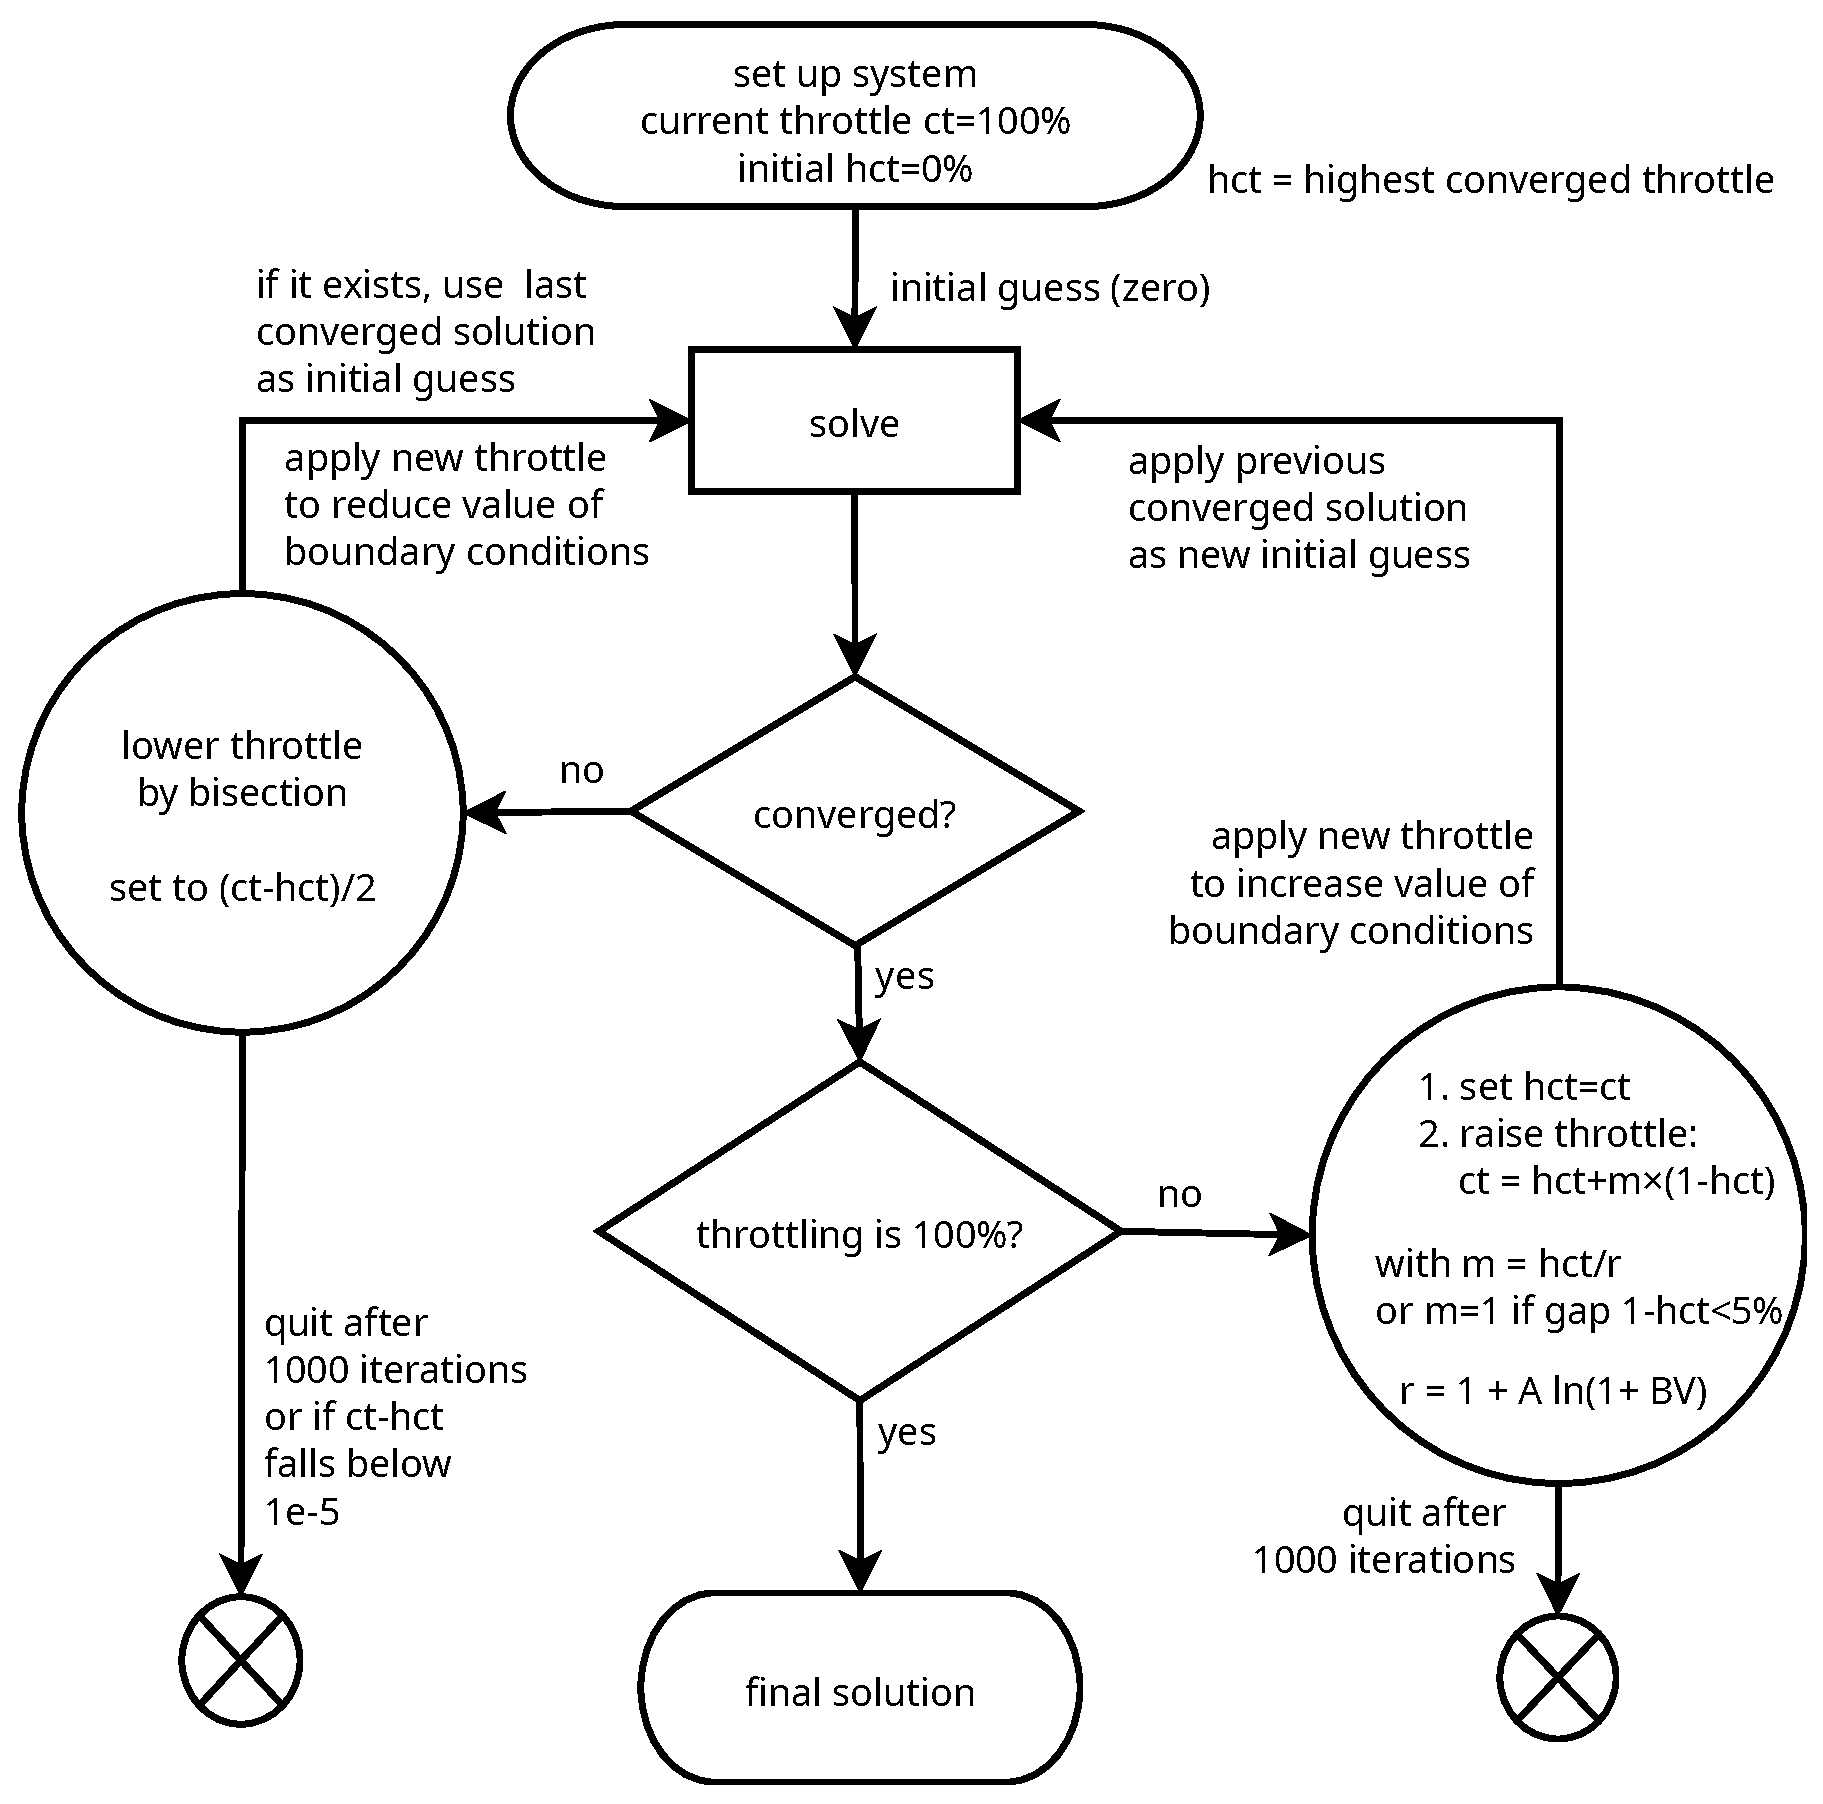
\includegraphics[width=1.1\linewidth]{throttling4.eps}
\caption{Flowchart for the throttling algorithm }
\label{fig:throttling_algorithm}
\end{figure}

The throttle is a multiplier
applied to the magnitude of the boundary conditions.
If the solver fails to converge, then we reduce the throttle downwards by
bisection between the current failed value (current throttle, ct) and the highest converged
throttle (hct, initially zero). Once the boundary
condition is throttled low enough to generate a converged solution,
we update the hct and raise
the throttle upwards by an amount $u$, closing the gap towards 100\% (we set the throttle
to 100\% if the procedure would exceed it).  The value of $u$
must find a balance between reaching a 100\% throttle in as few
iterations as possible (do not make $u$ too small), while not collapsing back to non-converging
conditions when raising the throttle (do not make $u$ too
large). Empirically, we find that, when the hct is small, the rise rate
must also be small to obtain the next converged iteration. Once the hct is
large, the rise rate may be proportionally larger. We therefore
propose a rise step $u=m\times (1- \mathrm{hct})$ such that the next
throttle applied after a converged iteration is
\begin{equation}
  \mathrm{ct [new]} = \mathrm{hct} + m (1-\mathrm{hct}),
\end{equation}
with
\begin{equation}
  m=
  \begin{dcases}
    \frac{\mathrm{hct}}{r} &, \\
    1 & \text{if } 1-\mathrm{hct} < 5\%.
  \end{dcases}
\end{equation}
This produces a quadratically accelerating rise rate and attempts a
direct jump to 100\% once the remaining gap is less than 5\%.  It is likely
that our formulation, quadratic in the hct term, approximates a more 
optimal exponential (or
sigmoidal) rise rate.

\subsubsection{Optimal Throttling}
An example of
the throttle rate against the number of iterations is presented in
Fig.~\ref{fig:throttle_rate} for 1 V and 10 V boundaries with different
choices of fixed values of the rise rate multiplier $r$. A best value of $r$ can be identified
for each voltage, minimizing the number of iterations required,
for example, $r=2$ for 1 V and $r=3$ for 10 V. A
value of $r$ larger than the best value means the rise step is
smaller, such that convergence is smooth, but requires more
iterations. A lower value of $r$ means the rise step is too large,
overstepping and resulting in a nonconverging iteration, such that
more iterations are required to fall back to a converging throttle rate.

\begin{figure}
\centering
(a)
\includegraphics[width=0.45\linewidth]{test_1V.eps}
(b)
\includegraphics[width=0.45\linewidth]{test_10V.eps}
\caption{Attempted throttle rate versus iteration numbers for (a) 1 V and
  (b) 10 V  boundaries with fixed rise rate multipliers $r=1,2,3$, and
  4. The steric model is solved with log-zero scaling.
}
\label{fig:throttle_rate}
\end{figure}

The best-performing fixed values of $r$  for potentials up to 100 V are presented 
in  Fig.~\ref{fig:best_throttle_rate}.  We observe a similar trend in 1D calculations with
trivial and log-zero function scaling  (the
differences may not be significant, since only integer values of $r$ up
to 10 were tested). A priori, we have no reason to expect the
optimal value of $r$ to be universal, and we might expect it to vary with
conditions such as the electrolyte concentration or
dimensionality. However, we plot the best $r$ values for trivial
scaling over a wide range of concentrations (1D calculations), as well as  2D and 3D calculations of the flat electrode (at a 1M
concentration). In all cases, the best $r(V)$  essentially follows the
same curve, with a small deviation seen only at 1--2 V, which can be attributed simply to the
integer resolution of the simulation.  The time per iteration varies with system conditions and
dimensionality, but the optimal $r(V)$ for minimizing the number of
iterations remains the same. The optimal $r(V)$ can be considered to be universal.



\begin{figure}
\centering
\includegraphics[width=0.8\linewidth]{best_r_vs_V.eps}
\caption{Best fixed rate multiplier $r$ for each voltage, with the lowest
  number of throttling iterations. The steric model is solved with both
  trivial (in black) and log-zero (orange dashed line) concentration scaling (1D calculation at a 1M
  electrolyte concentration).
  We also show the best $r$ values for 1D calculations with trivial scaling over a range of
  concentrations (blue stars)
  and 2D and 3D calculations (black boxes) of a flat electrode at
  a 1M concentration. The solid purple line denotes the model $r(V) = 1 +
  3.78 \ln(1 + 0.102 V)$ fitted to trivial scaling data. The grey lines
  mark uncertainty bounds of one standard deviation in the fitted parameters.
}
\label{fig:best_throttle_rate}
\end{figure}

\subsubsection{Adaptive Throttle Rate}
The trend in the best-performing $r$ values shown in Fig.~\ref{fig:best_throttle_rate} suggests that an
optimal multiplier follows
$r \propto \ln V$, indicating that $r$ 
may be tuned adaptively to provide the maximum possible rise rate (smallest
possible $r$) that minimizes the number of unsuccessful non-converged
attempts for the given boundary condition.  A milder
rise rate (larger $r$) is required at larger surface potentials.
Allowing for a finite value of $r$ when $V \rightarrow 0$, we propose
an adaptive definition of $r$,
\begin{equation}
  r(V) = 1 + A \ln(1 + B V).
  \label{adaptive_r}
\end{equation}
This model imposes the limit $r \rightarrow 1$ as $V \rightarrow 0$.
In principle, an optimal low-voltage multiplier might allow $r<1$ if
$r>$hct, but the limit of one is simpler, avoiding the need to 
compare against the hct. Fitting against the best $r$ values for trivial scaling
results in $A=3.78 \pm 0.36$ and $B=0.102 \pm 0.020 \textrm{ V}^{-1}$.
The uncertainties here have been determined from the covariance matrix
generated by the fitting procedure implemented in the
\verb|curve_fit| function provided by the \texttt{optimize} module in SciPy
\citep{VugrinSwilerRobertsStuckyMackSullivan2007}. 
 The best $r$ value for log-zero scaling is similar. One could separately fit
 parameters for log-zero scaling (to obtain 
 $A=1.3\pm 0.2$ and $B=0.7 \pm 0.5 \textrm{ V}^{-1}$).
 Nevertheless,  Fig.~\ref{fig:best_throttle_rate} shows that the
 log-zero data points lie only one standard deviation below the trivial
scaling fit. Statistically, there is no significant difference in the
best $r$ values for trivial and log-zero scaling.

We emphasize that the value of $V$ used in the adaptive $r$ formula, \eqref{adaptive_r},
must be the target boundary condition (the final electrode voltage),
and not the throttled boundary condition at the given iteration.  If a throttled $V$ were
applied, $r$ would be small when the boundary condition is strongly
throttled, resulting in large rise steps that lead to convergence
failure when the  target voltage is large.


Table~\ref{tab:convergence} shows  the number of iterations required
to converge with various boundary conditions for the different
concentration scaling functions in both the point charge model and the
steric model and applying an adaptive
$r(V)=1+3.78\ln(1+0.102V)$ for 1D meshes with 30 cells. For the point charge model, trivial scaling 
permits calculations only up to 0.7 V. Log scaling permits calculations up to 0.8 V, and log-zero
scaling permits calculations up to 1 V (1.5 V can be reached with a finer mesh).

\begin{table}
  \centering
  \begin{tabular}{c|ccc|ccc}
Pot. (V)  & \multicolumn{3}{c|}{Point Charge} & \multicolumn{3}{c}{Steric}    \\
        & Trivial & Log & Log-Zero & Trivial & Log & Log-Zero \\ \hline
%%%%%%%%%%%%%%%%%%%%%%%%%%%%%%%%%%%%%%%%%%%%%%%%%%%%%%%%%%%%%%%%%%%%%%
%%                                                                  %%
%%  This is a LaTeX2e table fragment exported from Gnumeric.        %%
%%                                                                  %%
%%%%%%%%%%%%%%%%%%%%%%%%%%%%%%%%%%%%%%%%%%%%%%%%%%%%%%%%%%%%%%%%%%%%%%
%NaCl 1M	&	&	&	&	&	&\\
%	&pot(x)/surf\_pot + non linear geometry 	&	&	&	&	&\\
%	&Steric OFF	&Steric OFF + log	&Steric OFF + log\_zero	&Steric ON	&Steric ON + log	&Steric ON + log\_zero\\
%Surface Potential [V]	&Throttle attempts	&	&	&	&	&\\
0.1	&1	&1	&1	&1	&1	&1\\
0.5	&1	&1	&1	&1	&11	&9\\
0.7	&6	&1	&1	&1	&11	&11\\
0.8	&S	&10	&6	&6	&11	&11\\
0.9	&	&S	&8	&1	&14	&12\\
1	&	&	&7	&1	&14	&12\\
1.1	&	&	&F	&7	&14	&14\\
1.5	&	&	&	&10	&15	&15\\
2	&	&	&	&8	&19	&16\\
5	&	&	&	&18	&27	&27\\
10	&	&	&	&27	&F	&39\\
100	&	&	&	&91	&	&114\\
%250	&	&	&	&240	&	&180\\
%375	&	&	&	&355	&	&212\\
%500	&	&	&	&419	&	&230\\
%625	&	&	&	&478	&	&321\\
%750	&	&	&	&517	&	&382\\
%875	&	&	&	&551	&	&428\\
1000	&	&	&	&439	&	&369    \\
2000	&	&	&	&S	&	&762    
  \end{tabular}
\caption{\label{tab:convergence}Number of throttling iterations
  required to  solve the PB model of a 1M NaCl electrolyte solution
  for various electrode potentials and concentration scaling
  functions (trivial, log, or log-zero scaling) for both the classic point charge model and the steric
 (Carnahan--Starling) model with finite ion sizes. The adaptive rise rate
  multiplier $r(V)=1+3.78\ln(1+0.102V)$ for a 1D mesh with 30 cells. 
  F = failed
  (throttle step $<10^{-5}$), and S = stopped at 1,000 iterations.}
\end{table}


Trivial scaling is successful for the steric model up to 1,000 V, while simple log
scaling fails at 10 V due to instability introduced by near-zero coion
concentrations.
Log-zero scaling enables calculations to 2,000 V
and higher, beyond the limit of trivial scaling.
The corresponding
performance plot of iterations versus voltage for the steric model
(with both trivial and log-zero scaling) is presented in Fig.~\ref{fig:convergence}.
 The steric model
naturally keeps concentrations within 
physically reasonable bounds, such that  log-zero scaling is not
required for normal electrochemical conditions. 
Trivial scaling performs better than log-zero scaling when $V<100$ V,
the region of electrochemical interest.
Performance is robust with respect to the $A$ and $B$ parameters used to
determined $r(V)$, whether fitted to the best $r$ for trivial or log-zero scaling.
2D and 3D calculations generally require the same number of iterations
as 1D calculations, showing small differences only at 1--2 V.
Even with log-zero scaling, computation of the interaction of
100 kV electrical transmission cables with saline water would require
such a large number of iterations that this algorithm would become impractical.

\begin{figure}
\centering
\includegraphics[width=0.8\linewidth]{num_attempts_vs_V.eps}
\caption{Number of throttling iterations, as a function of electrode
  voltage, needed to solve the steric model with trivial and log-zero scaling.  An adaptive rise rate multiplier
  $r(V)=1+3.78\ln(1+0.102V)$ is used to best fit trivial scaling (solid
  lines). 1D calculations with trivial scaling are shown in black,
  and log-zero scaling in orange. The rise rate $r(V)=1+1.3 \ln(1+0.7V)$
  (fitted for the best log-zero value) is also shown (dashed lines) for
  comparison. 2D data points are indicated by squares (trivial scaling) and
  diamonds (log-zero scaling). 3D data points (trivial scaling) are
  denoted by blue crosses.
}
\label{fig:convergence}
\end{figure}


The sample results of the adaptive throttling algorithm for an electrode charged to
10 V with Carnahan--Starling steric forces are presented in
Fig.~\ref{fig_results_throttling}, calculated with trivial scaling of the
concentration functions with adaptive $r$ coefficients $A=3.78$ and $B=0.102 \textrm{ V}^{-1}$).
Figure~\ref{fig_results_throttling}(b) shows the onset
of a steric adsorption layer \citep{DagmawiParsons2022} with counterion
concentrations constrained below a concentration cap determined by the
ion size, a cap of 46 mol/L in the case of our {Cl}$^{-}$ ion.

\begin{figure}
\centering
(a)
\includegraphics[width=0.45\linewidth]{steric_potential_10V.eps}
(b)
\includegraphics[width=0.45\linewidth]{steric_10V_counterion.eps}
\caption{\label{fig_results_throttling}Solutions to the modified
  PB model of a 1M NaCl electrolyte solution with
  Carnahan--Starling steric forces, shown as profiles along $x$, the
  perpendicular distance from a 10 V electrode surface. (a) Electrostatic
  potential. (b) Counterion ({Cl}$^{-}$) concentration. }
\end{figure}

\section{Conclusion}

Modelling complex electrolyte solutions in electrochemical conditions
with electrode potentials of 1 V or greater requires both nontrivial
physics and nontrivial numerical algorithms.
With respect to the
physics, aside from redox chemistry and electrolysis (not considered
here), the finite sizes of ions must be considered via
steric forces. These are expressed as a steric contribution to the
chemical potential of ions and used in the underlying thermodynamic
energy functional that provides the origin of the weak and strong
formulations of the system.
To achieve numerical convergence, we propose two
steps. First, we propose log-zero function scaling of
concentration functions that accounts
not only for the heightened concentrations of counterions near an
electrode, but also the near-zero concentrations of coions. Second and more importantly, we propose an adaptive throttling algorithm (a kind of homotopy
method) that reduces boundary conditions 
down to the linear regime, where a solution is easily obtained, and then
progressively propagates that solution by releasing the throttle
until the target boundary condition is obtained. Optimized convergence
is obtained by adaptively controlling the rise rate of the throttle factor
depending on the target boundary condition.

The combination of
log-zero scaling and throttling facilitates calculations of point
charge models up to 2 V. Log-zero scaling enables
the steric model to reach electrode potentials greater than 2,000 V. However, for typical electrochemical applications with potentials lower than 20 V,
where steric forces are needed to maintain the physical relevance
of the model, trivial scaling is sufficient and faster than log-zero scaling.
The empirical parameters for optimal throttling, minimizing the number of
required iterations, appear to be universal, independent of
the electrolyte concentration or whether the geometry is 1D, 2D, or 3D.
This might indicate a deeper structure in the algorithm that could be
revealed with further mathematical analysis. Our 1D, 2D, and 3D
simulations tested the same flat electrode surface. We expect the optimal throttling
conditions will continue to be valid with more complex 3D or 2D
geometries, though it may be prudent to confirm this assumption.

We illustrated the throttling algorithm using Dirichlet boundary
conditions (electrode potentials), but the  principle applies
equally to Neumann and more complex boundary conditions.

\begin{acknowledgement}
  We acknowledge the support of a CINECA award under the ISCRA
  initiative, for the availability of high-performance computing
  resources and support.

  A Python script demonstrating the throttle algorithm is available on Zenodo at \url{https://doi.org/10.5281/zenodo.14829963}.

\end{acknowledgement}

\bibliographystyle{spbasic}
% Write the full path of your bibfile relative to book.tex
\bibliography{chapters/parsons/bibliography.bib}
